%Template v.1.0: Taylor Arnold and Simon Gabay, december 2025
% CECI EST UN FICHIER DE MODÈLE LATEX POUR LES ARTICLES INCLUS DANS
% *Anthology of Computers and the Humanities*. AJOUTEZ L'OPTION
% 'final' LORS DE LA CRÉATION DE LA VERSION FINALE DE L'ARTICLE. 
% NE PAS modifier la classe du document

\documentclass[final, fra]{anthology-ch}     % pour la version finale
%\documentclass[fra, custom]{anthology-ch}      % pour la soumission

% CHARGER LES PACKAGES LaTeX
\usepackage{booktabs}
\usepackage{graphicx}



\title{Structuration, exploration et valorisation d'archives archéologiques par l’intelligence artificielle au sein d’un lac de données}

\author[1]{Rajae El-Idrissi}[
  orcid=0009-0008-9705-3550,
  email=rajae.el-idrissi@univ-lyon2.fr
]
\author[2]{Josefina Simon Reig}[
  orcid=0000-0002-8327-8133,
  email=josefina.simon.reig@gmail.com
]
\author[2]{Laura Romero}[
  orcid=0009-0002-2085-8461,
  email=lromero@gencat.cat
]
\author[1]{Juba Agoun}[
  orcid=0000-0003-4911-0617,
  email=juba.agoun1@univ-lyon2.fr
]
\author[3]{Jean-Pierre Girard}[
  orcid=0000-0003-4225-8678,
  email=jean-pierre.girard@mom.fr
]
\author[2]{Gabriel de Prado}[
  orcid=0000-0002-1408-1361,
  email=gdeprado@gencat.cat
]
\author[1]{Jérôme Darmont}[
  orcid=0000-0003-1491-384X,
  email=jerome.darmont@univ-lyon2.fr
]

\author[1]{Sabine Loudcher}[
  orcid=0000-0002-0494-0169,
  email=sabine.loudcher@univ-lyon2.fr
]
\affiliation{1}{Université Lumière Lyon 2, ERIC, Lyon, France}
\affiliation{2}{Musée d’Archéologie de Catalogne, Site d’Ullastret, Espagne}
\affiliation{3}{Université Lumière Lyon 2, Archéorient, Lyon, France}
 

% MOTS-CLÉS
% Fournissez un ou plusieurs mots-clés séparés par des virgules
% en utilisant les commandes suivantes
\keywords[fra]{archéologie, science des données, lac de données, métadonnées, carnets de fouille}
\keywords[eng]{archaeology, data science, data lake, metadata, excavation diaries}

\pubyear{2026}
\pubvolume{4}
\pagestart{182}
\pageend{188}
\paperorder{22}
\conferencename{Actes de la Conférence Humanistica}
\conferenceeditors{Serena Crespi, Simon Gabay, Martin Grandjean, Ariane Pinche, Marie Puren et Léa Saint-Raymond}
\doi{10.63744/B2JRjY8IpI43}
\customhead{}

\addbibresource{bibliographie.bib}

%%%%%%%%%%%%%%%%%%%%%%%%%%%%%%%%%%%%%%%%%%%%%%%%%%%%%%%%%%%%%%%%%%%%%%%%%%%
% DÉBUT DU TEXTE
\begin{document}

\maketitle

\begin{abstract}
The DataLAC project focus on the use of artificial intelligence for the alignment, annotation and interpretation of heterogeneous documents enriched with semantic metadata and aggregated within a data lake. This project seeks to digitize, unify and make accessible over thirty years of field notes (1947–1977), scientific publications, and archives related to the Iberian archaeological site of Ullastret.These diverse materials are integrated into an interoperable data lake designed to manage the heterogeneity of sources and to support complex research queries. The DataLAC project thus constitutes a generalizable proof of concept, demonstrating the potential of data lake architectures and AI-driven methodologies for the exploitation and interpretation of archaeological archives.
\end{abstract}
\vspace{1cm}

\section{Introduction}
Alors que les premiers archéologues consignaient leurs observations principalement dans des carnets manuscrits, les protocoles actuels reposent sur des formulaires et des systèmes numériques de gestion de données. Toutefois, il n’existe pas encore de standard pour ces données : aucun consensus ne s’est imposé concernant les systèmes d’information archéologique, les outils utilisés (tableurs, bases FileMaker, bases relationnelles propriétaires ou open source, etc.) ni les pratiques de modélisation des données, malgré des méthodes de terrain relativement homogènes. 
La recherche archéologique repose également sur la comparaison d’artefacts présentant des caractéristiques similaires, à partir de photographies, d’illustrations ou de croquis issus de carnets de terrain. L’automatisation de l’analyse de ces corpus constitue un défi majeur, nécessitant des techniques de reconnaissance graphique appliquées à des archives scientifiques très hétérogènes (carnets numérisés, inventaires, dessins, cartes, plans). Idéalement, il faudrait aussi pouvoir interconnecter l’ensemble des données archéologiques (qu'elles soient manuscrites ou nativement numériques) afin de disposer d’une vision complète et cohérente du processus de fouille archéologique.


Le projet DataLAC vise à relever une partie de ces défis sur un site ibérique de la première moitié du \textsc{vi}\textsuperscript{e}~siècle av. J.C. , le site d'Ullastret en Catalogne. Ce site est fouillé de façon continue depuis 1947 mais les documents des trente premières années de fouille ne sont pas numériques et ils sont très hétérogènes (cahiers de fouille, archives photographiques, inventaires des objets découverts). Ils posent d’importants défis en matière de numérisation, de reconnaissance d’écriture manuscrite et de mise en relation sémantique.

Pour maîtriser l'hétérogénéité de la documentation du site, pour faciliter le partage et l’analyse des données, le projet DataLAC mobilise le concept de lac de données qui vise à conserver ces dernières dans leur forme/format originel(le). Elles demeurent ainsi, à condition d’être soigneusement documentées par des métadonnées, des références mobilisables. La modélisation des métadonnées décrivant les entités de données d’un lac de données est cruciale et elle doit être assortie d'un système de gestion des métadonnées efficace pour permettre une interrogation et une analyse efficaces des données hétérogènes. 


En d'autres termes, le projet DataLAC vise à développer une preuve de concept pour exploiter et analyser des corpus archéologiques en mobilisant des outils de science des données au sein d'un lac de données intégrant des sources hétérogènes et métadonnées.

Pour atteindre son objectif le projet DataLAC comprend quatre phases : 
\begin{enumerate}
    \item La numérisation des treize cahiers de fouilles manuscrits et de toute la documentation scientifique (rapports, photos, diapositives, plans, etc.). L'ensemble des documents numérisés constitue le corpus du projet.
    \item La transcription automatique des 4000 pages des treize carnets grâce à la reconnaissance automatique d’écriture manuscrite à l'aide de modèles d'intelligence artificielle. 
    \item La modélisation et l'enrichissement des métadonnées décrivant les documents numérisés. Chaque carnet, page, ligne, document scientifique est décrit par plusieurs métadonnées. Ces dernières sont mises en relation grâce à un thésaurus archéologique multilingue permettant de produire des métadonnées normalisées et interrogeables.
    \item L'interrogation sémantique. Les documents et leurs  métadonnées sont organisés dans un lac de données et sont accessibles via un système de gestion des métadonnées composé d'une base de données relationnelle, d'une API et d'une interface Web pour faciliter la recherche, la visualisation et l'annotation des documents du corpus.
\end{enumerate}

La suite de l'article présente chacune de ces phases.

\section{Corpus et thésaurus} 
\label{sect:corpus}

Le corpus du projet rassemble des archives qui retracent trois décennies de fouilles archéologiques du village ibérique de Puig de Sant Andreu à Ullastret\footnote{\url{http://www.macullastret.cat}.}. Au cœur de cette collection se trouvent treize carnets de terrain manuscrits, rédigés entre 1947 et 1977, en catalan et en castillan, par l'archéologue Miquel Oliva i Prat et ses collaborateurs. Leur contenu se distingue par une grande hétérogénéité : quelques 4000 pages mêlent observations narratives, annotations techniques, croquis d’artefacts ou de fouilles, diagrammes stratigraphiques, plans de fouilles et notes de terrain provisoires. À ces carnets s’ajoutent de nombreux feuillets supplémentaires, manuscrits ou dactylographiés, insérés au fil des carnets. Ces documents additionnels incluent, des photographies de terrain ou encore des matériaux éphémères produits au cours des campagnes de fouilles.

En plus des carnets, le corpus comporte également des dessins techniques (relevés de terrain, planches de profils de céramiques), des photographies techniques (vestiges sur le terrain, couches stratigraphiques, planches d’objets), des cartes et plans de diverses époques. Tous ces documents représentent les excavations, les artefacts, les contextes de terrain et les archéologues au travail. L'ensemble a été numérisé par le musée-site d'Ullastret et mis à disposition du projet. 

Chaque carnet, page de carnet, croquis, feuillet supplémentaire, photo, plan, etc. est décrit par un ensemble de métadonnées.  Une première catégorie de métadonnées est directement extraite des signatures techniques embarquées dans les fichiers résultant de la numérisation ; ces métadonnées primaires ne suffisent pas, elles doivent être enrichies de sémantique permettant de décrire finement le contenu des carnets et des documents scientifiques (« \textit{ce document représente cet artefact} » ou « \textit{cet artefact est dans la zone A fouillée par Oliva, zone qui correspond aux zones modernes X et Y} ») ou permettant de faire également des liens entre tous les documents du corpus (« \textit{ces deux documents décrivent le même artefact} »). Les archéologues impliqués dans le projet DataLAC
ont défini un ensemble de descripteurs terminologiques fondés sur le vocabulaire utilisé dans les carnets de fouille, descripteurs qui permettent d'annoter les pages des carnets. Ils constituent des métadonnées riches sémantiquement et sont organisés dans un thésaurus\footnote{\url{https://thesaurus.mom.fr/?idt=th62}.} bilingue (catalan-castillan, qui sera ultérieurement apparié avec des concepts en français). Ce thésaurus constitue un outil d'une part pour l'annotation sémantique et pour la normalisation terminologique des descripteurs, d'autre part par les relations logiques qu’il introduit entre les labels des différents de concepts identiques ou proches. A terme il sera aligné sur les références archéologiques, contribuant ainsi à l'interopérabilité du corpus du projet.


\section{Segmentation et transcriptions automatiques des carnets} 
\label{sect:transcription}
La transcription automatique des pages des carnets de fouille comporte deux étapes : (1) extraction et structuration des éléments graphiques pour reconnaître les positions des lignes de texte, des illustrations (\textit{e.g.,} des croquis) et des zones vierges dans les pages des carnets ; (2) production d'une transcription exploitable des lignes de texte (figure~\ref{seg_trans}). Ce processus de reconnaissance de l’écriture manuscrite (ou HTR pour \textit{Handwriten Text Recognition}) s'appuie sur des modèles d'apprentissage automatique affinés.

\begin{figure}[!h]
\begin{center}
 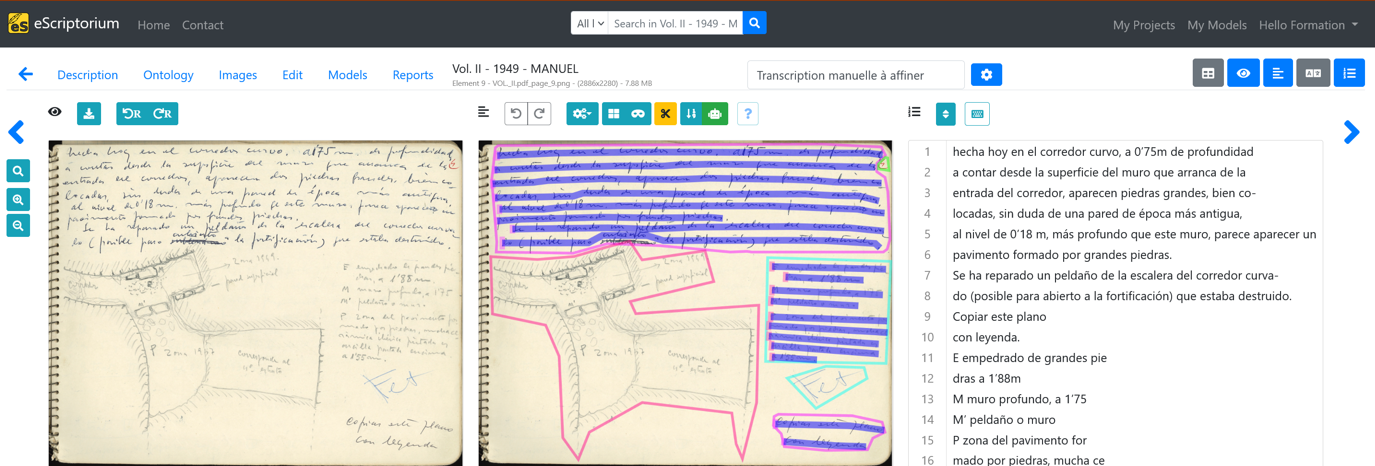
\includegraphics[scale=0.5]{img/Segmentation_transcription.png}
 \caption{Segmentation et transcription des pages des carnets de fouille.} \label{seg_trans}
\end{center}
\end{figure}

Toutes les opérations de segmentation et de transcription sont effectuées à l’aide de l'application \texttt{eScriptorium}\footnote{\url{https://escriptorium.rich.ru.nl/} et \url{https://gitlab.com/scripta/escriptorium}.} et du moteur d'HTR \texttt{Kraken}. Deux modèles pré-entraînés ont servi de point de départ avec un spécialisé dans la segmentation des zones de texte et des lignes, et l'autre pour la transcription des zones segmentées. Les transcriptions obtenues sont exportées au format XML ALTO, avec des balises conformes aux principes de l’ontologie \texttt{SegmOnto}\footnote{\url{https://segmonto.github.io}.} \cite{Gabay024}.

\subsection{Segmentation des pages}
Le modèle de segmentation \texttt{blla.mlmodel} est utilisé pour identifier automatiquement les lignes de texte dans les pages des carnets \cite{kiessling2020}. Ce modèle\footnote{\url{https://zenodo.org/records/14602569}.}, à base de réseaux de neurones convolutifs (CNN), est le modèle de segmentation de \texttt{Kraken} pré-entrainé à l'aide de toutes les données de Gallicorpora\footnote{\url{https://github.com/Gallicorpora/Segmentation-and-HTR-Models}.}.


Appliqué sur les pages des carnets de fouille, le modèle n'arrive pas à distinguer correctement les zones non textuelles, en particulier les illustrations (croquis, photos collées, plan manuscrit) et les zones vierges dans les pages. Une correction manuelle est nécessaire pour ajuster les résultats de segmentation aux besoins spécifiques du projet, à savoir l’ajout de zones graphiques et de zones vides (figure~\ref{seg_trans}). Ces corrections, réalisées sur les zones segmentées par le modèle de quatre carnets, permettent de constituer un jeu de données d’entraînement de 364 pages visant à affiner le modèle de segmentation \texttt{blla.mlmodel}. L’entraînement, réalisé sur une GPU, a nécessité environ 7 heures de calcul. Estimée par validation croisée, la proportion de pixels correctement classés est de 97,2\%.

%Pour garantir une conformité maximale aux standards d’annotation adoptés, le tag \colorbox{Periwinkle}{Text} (présent dans le modèle initial) est fusionné avec le tag \colorbox{Lavender}{MainZone} afin d’harmoniser la sortie du modèle avec la structure exigée par l’ontologie \texttt{SegmOnto}. Durant la phase d'entraînement, nous avons utilisé l'option \texttt{resize new} pour ajuster dynamiquement la couche de sortie du modèle et ne conserver que les tags présents dans les données d’entraînement, éliminant ainsi les tags non représentés dans le corpus. Ceci améliore la cohérence du modèle et réduit le bruit lors de la prédiction.
Le score moyen d’intersection (\textit{Intersection over Union} IoU) vaut 36,6\%, une valeur relativement faible, expliquée par la formation de contours flous autour des zones. En effet, les carnets contiennent de petites lignes de quadrillage qui introduisent probablement du bruit dans le processus de détection des zones. Néanmoins, le modèle conserve une bonne performance globale et assigne correctement les nouveaux labels aux zones détectées. Néanmoins, l’IoU pondéré atteint 79\%, indiquant une bonne performance globale du modèle notamment pour la zone principale contenant les lignes de texte. % notamment pour les classes principales telles que les \colorbox{Lavender}{MainZone}.

Le modèle affiné est ensuite appliqué sur le reste des carnets pour segmenter toutes leurs pages puis les erreurs produites sont corrigées manuellement. Même si le modèle affiné produit encore des erreurs, son utilisation (comparée à celle du modèle non affiné) permet de réduire quand même significativement le temps nécessaire pour corriger les positions des différentes zones segmentées.


\subsection{Transcription des pages}
La phase de transcription automatique débute par l’application du modèle \texttt{Manu~McFrench}\footnote{\url{https://zenodo.org/record/6657809}.} à toutes les zones de texte segmentées \cite{chague2023}. Ce modèle a été retenu car il a été pré-entraîné sur un corpus de manuscrits écrits en français, en espagnol ou en anglais, sachant que peu de modèles de transcription sont pré-entraînés sur des manuscrits écrits en espagnol et encore moins en catalan.
Sur la base de 589 pages transcrites manuellement des quatres carnets, le modèle \texttt{Manu~McFrench} est affiné. L’option \texttt{resize new}, option spécifique à \texttt{Kraken}, est activée pendant l’entraînement pour ajuster dynamiquement la couche de sortie du modèle et n'inclure uniquement les caractères présents dans les données d’entraînement, éliminant ainsi les glyphes non représentés dans le corpus. Cela améliore la cohérence typographique du modèle et réduit le bruit lors de la prédiction.
L’évaluation du modèle affiné a donné des résultats globalement satisfaisants. Le taux moyen de reconnaissance des caractères, estimé par  validation croisée, a atteint 90,6\%, tandis que le taux de reconnaissance des mots, plus strict, s’est établi à 67,8\%. Cette différence, attendue lors du traitement de textes manuscrits, est due à la sensibilité accrue de la seconde métrique aux erreurs ponctuelles : une seule lettre incorrecte peut invalider un mot entier. Malgré ces limites, les performances obtenues confirment l’adéquation du modèle pour une application à grande échelle. Son utilisation sur les carnets restants accélère significativement la transcription des pages, mais sur une phase de correction a posteriori reste nécessaire. 
Il est important de rappeler que l’objectif n’est pas seulement d’obtenir les meilleures performances possibles, mais de produire une transcription complète de toutes les pages des carnets. Il a fallu trouver un équilibre entre le temps consacré à la transcription manuelle des premiers carnets, celui à l’amélioration des modèles et celui nécessaire à la correction des erreurs. Ce processus a réduit de manière significative le temps requis pour la transcription et la localisation des différentes zones d’intérêt, une tâche qui aurait été beaucoup plus chronophage si elle avait été réalisée entièrement à la main.

\section{Lac de données} \label{sect:lac}
Pour lever les verrous informatiques liés au stockage, à l’interrogation, à l’analyse et à la visualisation des données hétérogènes, le projet utilise le concept de lac de données qui propose de stocker les données dans leur format d’origine, sans schéma prédéfini et sans transformation préalable à leur stockage \cite{dixon2010, hai2016}. Avec un tel principe, tous types de données peuvent cohabiter dans un lac de données, qu'elles soient structurées ou non. Toutefois, pour être exploitable, un lac de données a besoin de métadonnées qui permettent de décrire et de relier les entités de données stockées dans le lac, ainsi que d'un système efficace de gestion de ces métadonnées. 

\subsection{Système de gestion des métadonnées}

%Dans des travaux antérieurs au projet DataLAC, nous a étendu la définition du concept de lac de données, ainsi que les fonctionnalités qu’un système de gestion de métadonnées doit avoir pour être complet et efficace \cite{sawadogo2019}. De plus, nous avons proposé un méta-modèle~\cite{scholly2021} de métadonnées qui comprend trois niveaux de modélisation (conceptuel, logique et physique). 
Dans le projet, nous utilisons la définition du concept de lac de données ainsi que les fonctionnalités, qu’un système de gestion de métadonnées doit avoir pour être complet, que nous avons proposées dans des travaux antérieurs \cite{sawadogo2019, scholly2021}.

\begin{figure}[!htp]
\begin{center}
 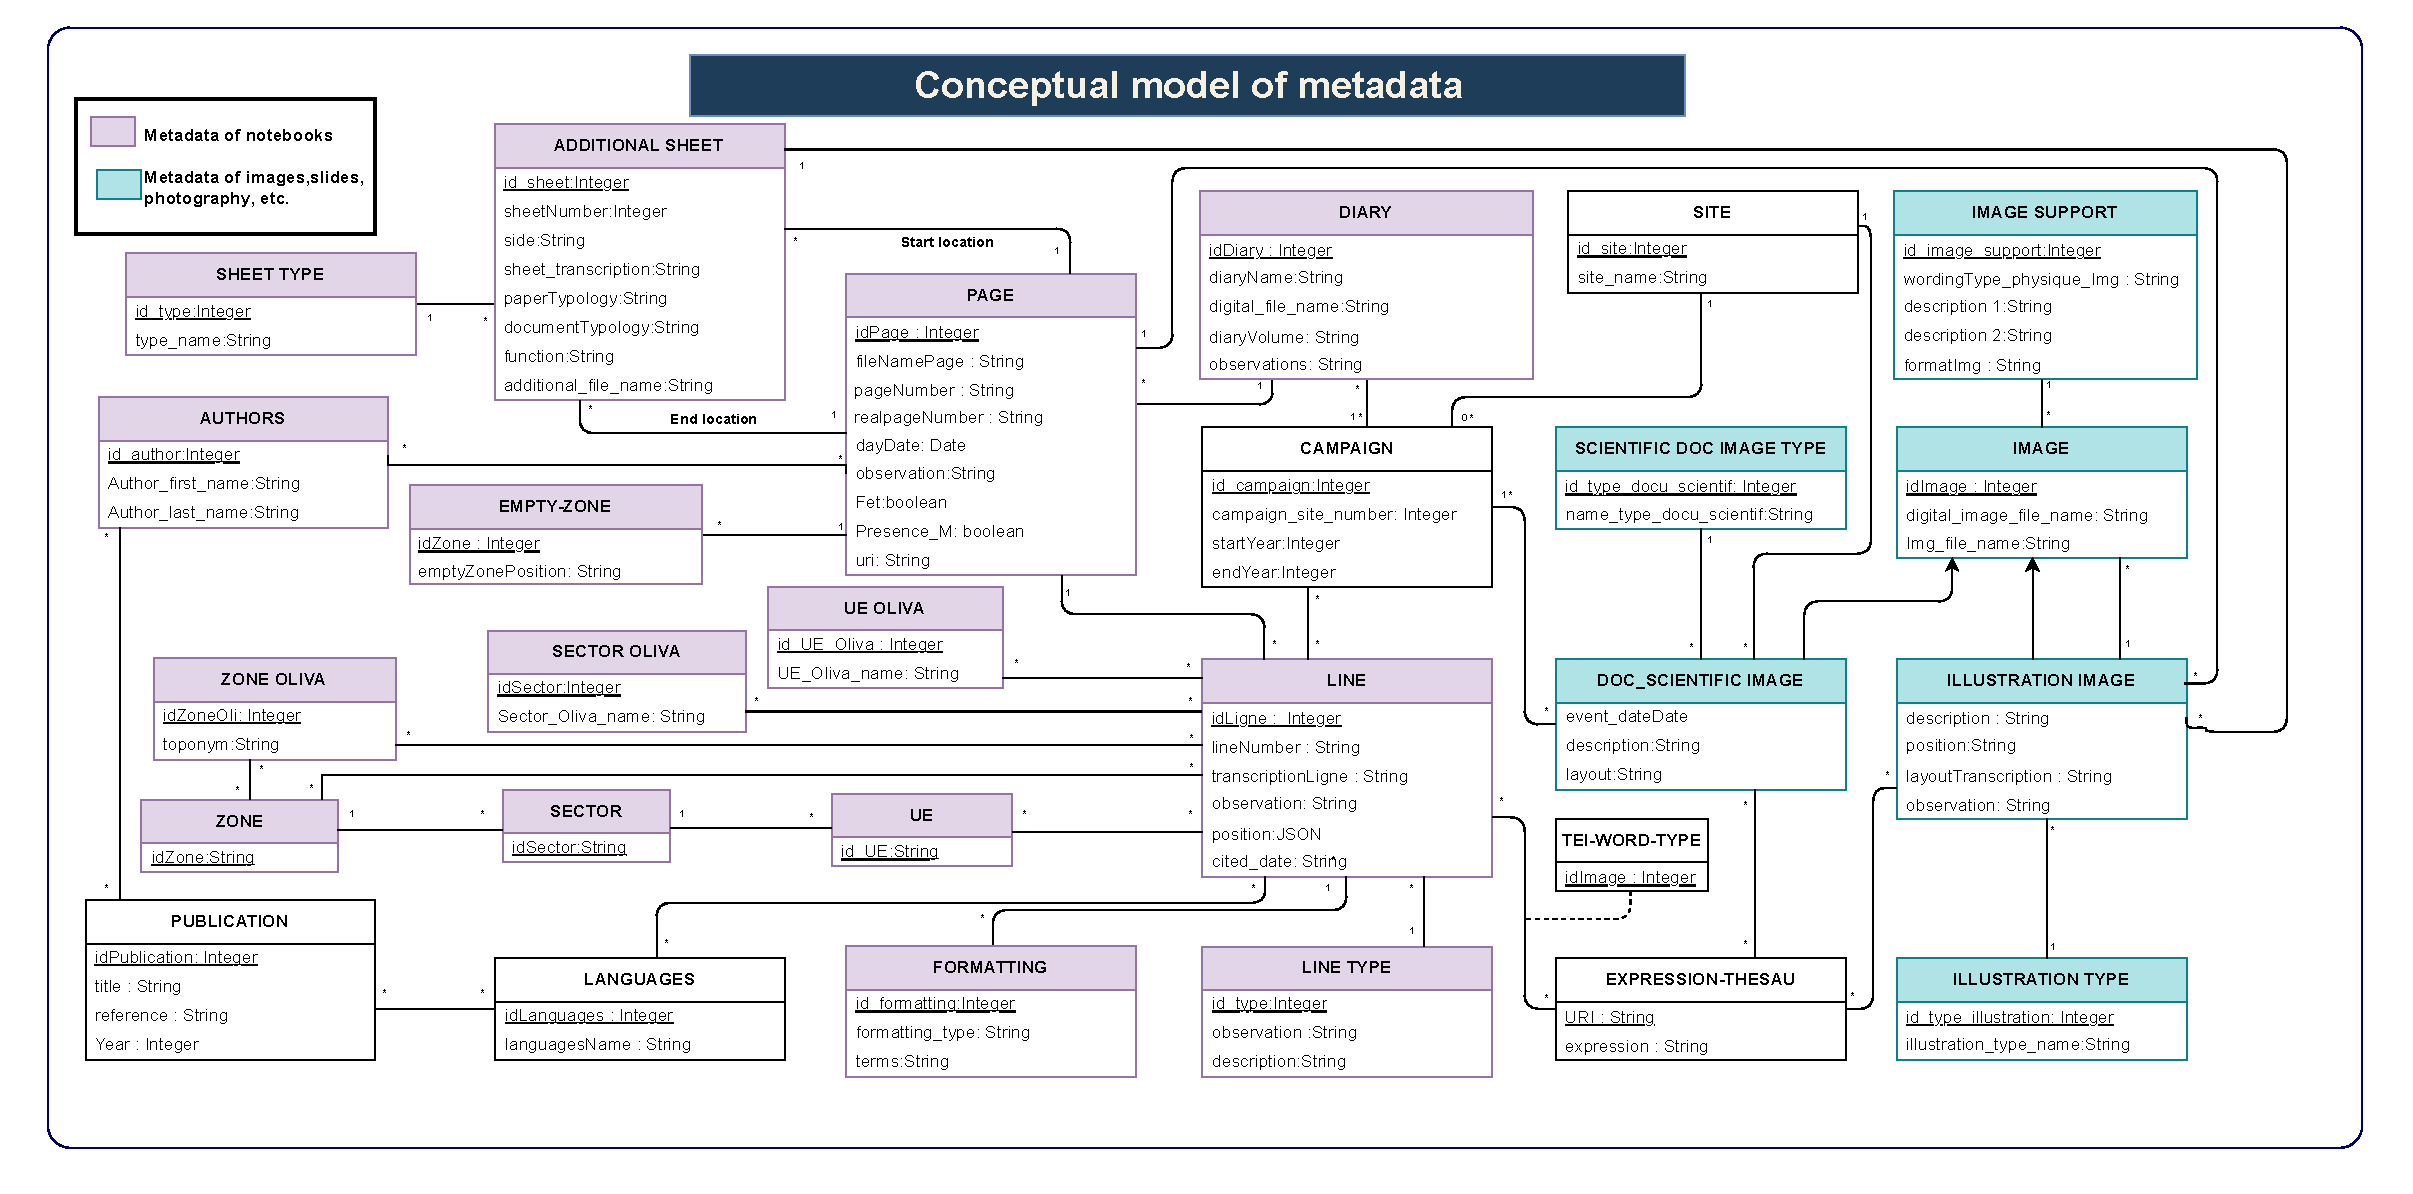
\includegraphics[width=\linewidth]{img/MCD_version_presentable.pdf}
 \caption{Modèle conceptuel des métadonnées.} \label{MCD}
\end{center}
\end{figure}


La figure~\ref{MCD} représente le modèle conceptuel des métadonnées décrivant tous les documents numérisés à savoir les carnets, leurs pages, les illustrations et feuilles supplémentaires présentes dans les carnets ainsi que toute la documentation scientifique. Chaque type de document correspondant à une classe dans le modèle conceptuel avec les attributs appropriés. La transcription automatique de chaque ligne de texte des pages est dans la classe ligne. 
Les mots-clés, désignés par \textit{expression-thesau} dans la figure~\ref{MCD}, sont piochés dans le thésaurus et décrivent sémantiquement tous les documents. Les zones, secteurs et unités stratigraphiques d'Oliva permettant de localiser les descriptions faites dans les lignes des pages  sont également dans le thésaurus. 

Ainsi toutes les documents du corpus sont décrits par une série de métadonnées et le thésaurus permet de les relier entre elles.




\subsection{Architecture du lac de données}
\begin{figure}[!htp]
\centerline{
 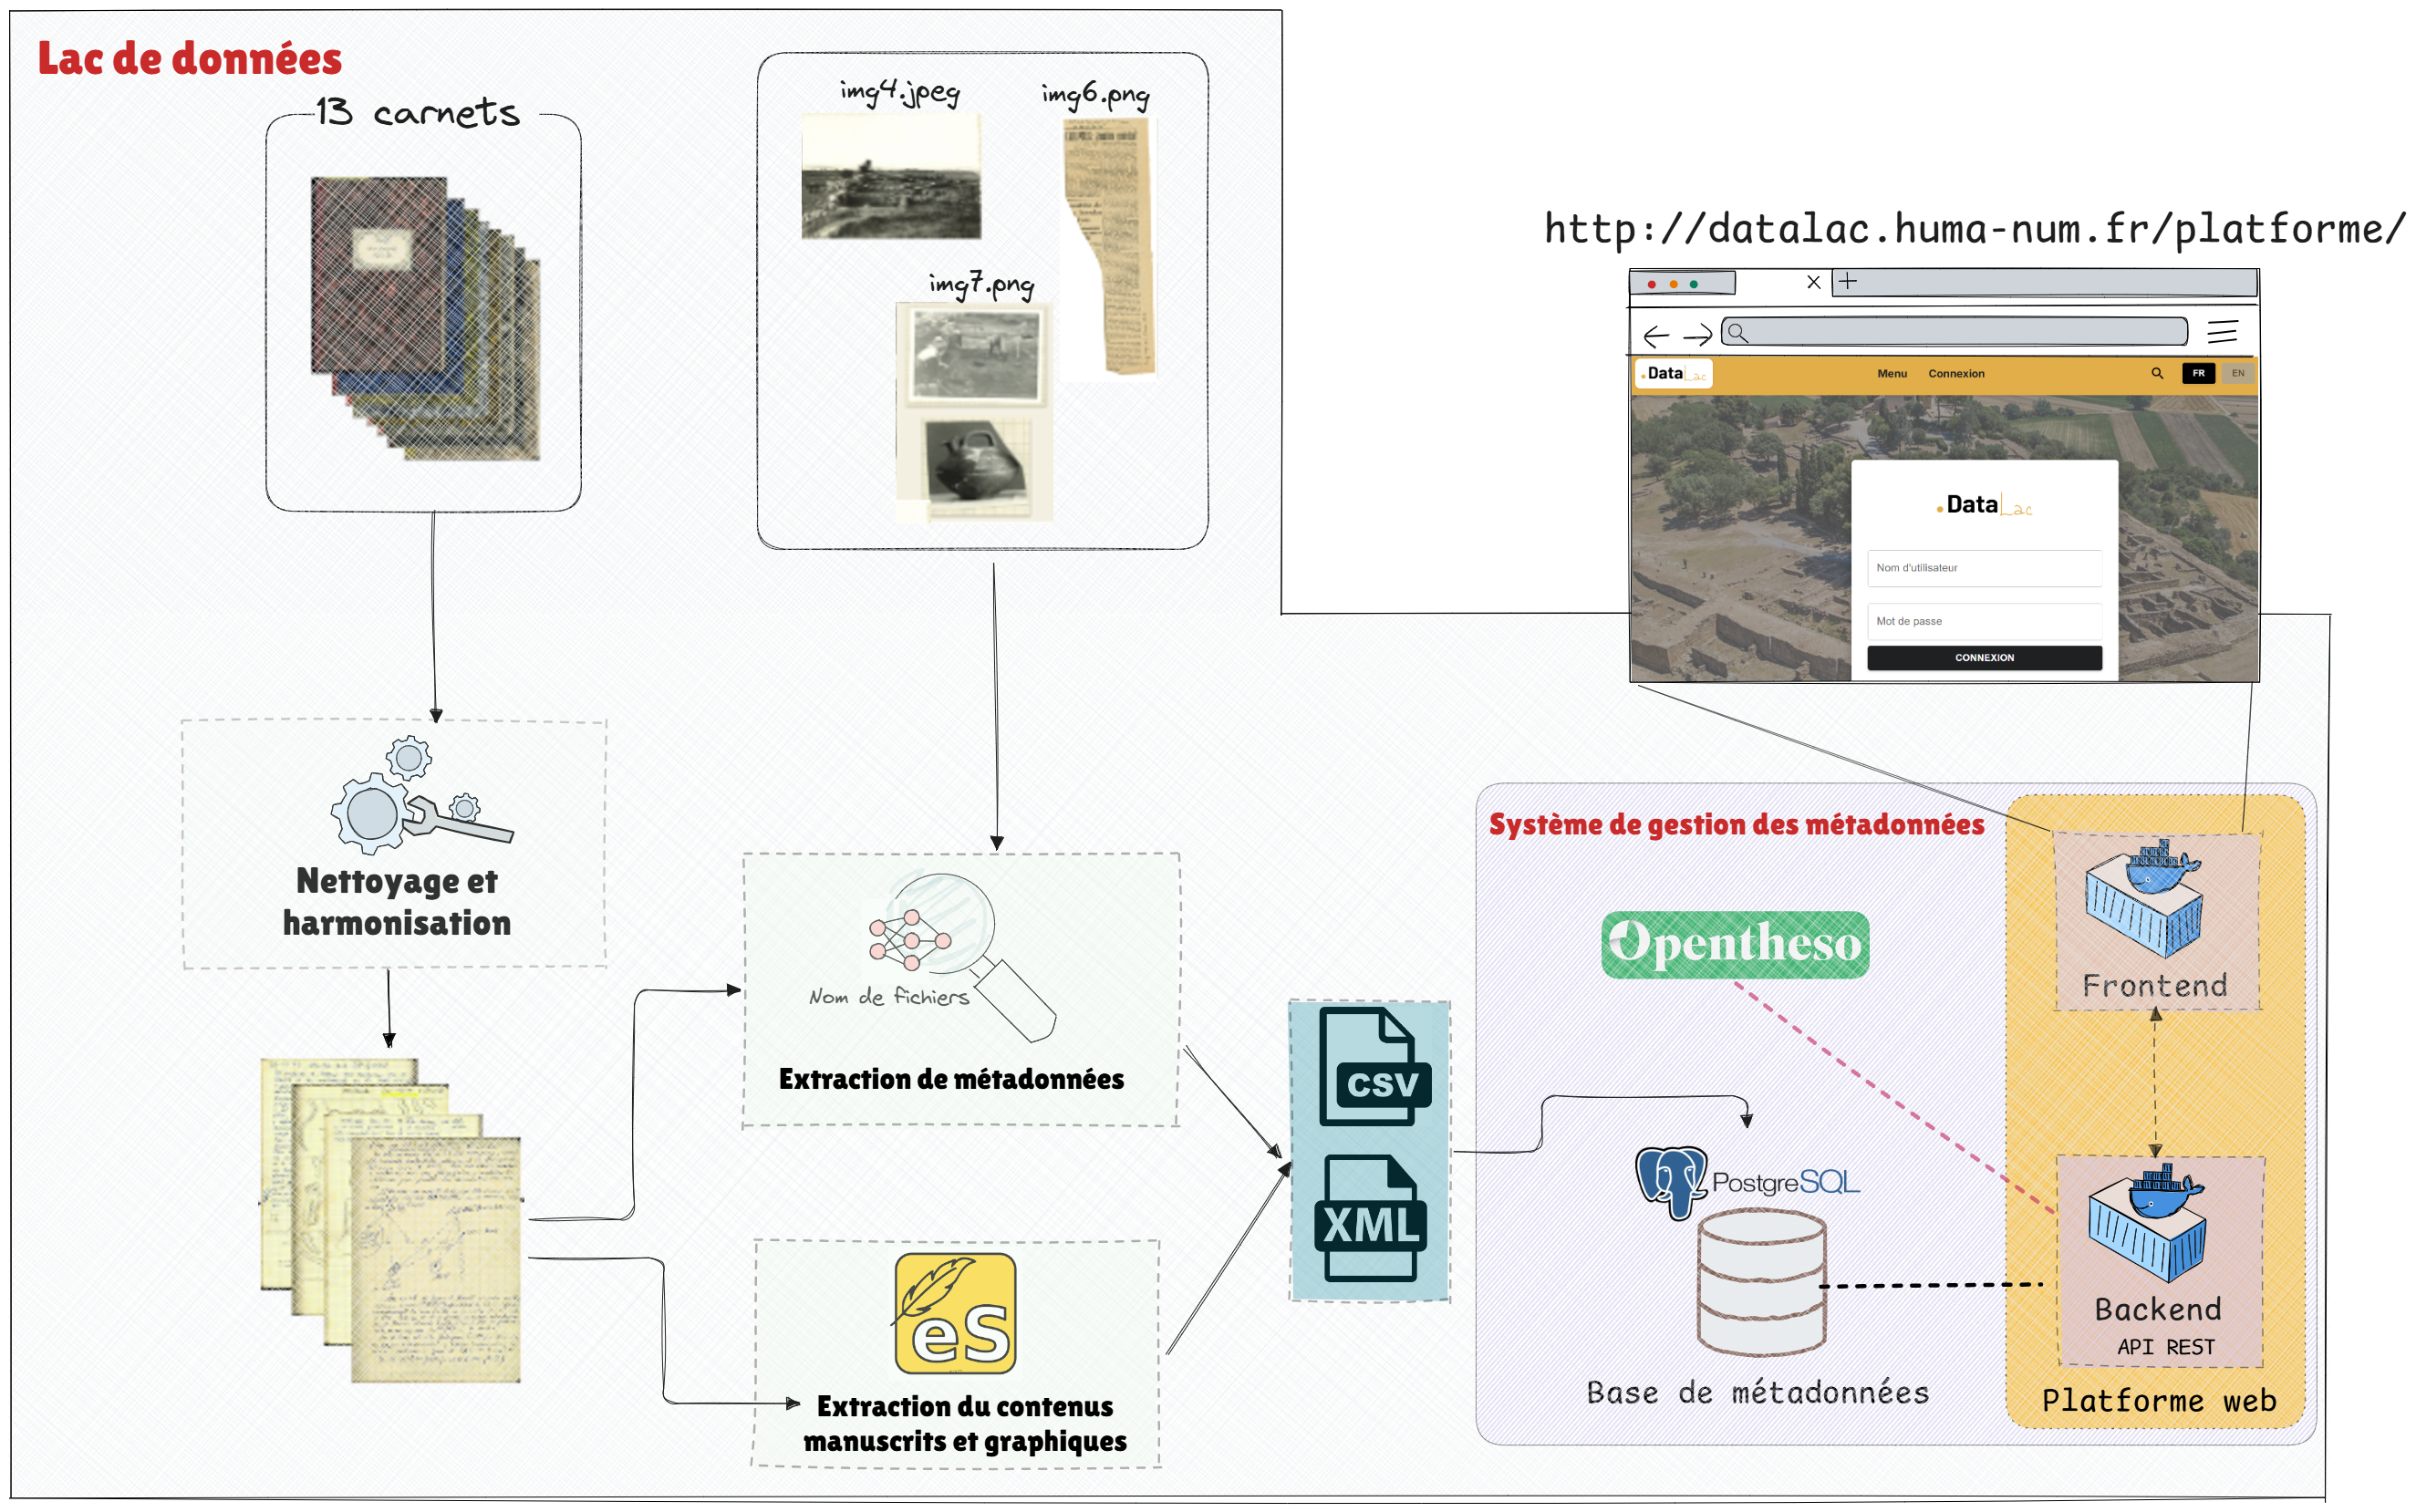
\includegraphics[width=\linewidth]{img/datalac-archi-egc.png}}
 \caption{Architecture du lac de données.} \label{Architecture}

\end{figure}

Le système de gestion des métadonnées comprend une interface Web conçue pour la saisie/modification, la consultation et la mise en relation des métadonnées des documents du corpus (figure~\ref{Architecture}). L'interface communique avec le back-end via une API RESTful. Les métadonnées sont stockées dans une base de données relationnelle PostgreSQL. 
Le thésaurus, hébergé sur la plateforme Opentheso\footnote{\url{https://thesaurus.mom.fr/?idt=th62}.}, est intégré dans le système de gestion de métadonnées. Cette architecture modulaire permet non seulement d'avoir un système efficace de gestion des métadonnées, mais elle soutient également de futures évolutions, telles que l’intégration de nouveaux types de documents, l'alignement du thésaurus sur des référentiels archéologiques et le développement d’outils analytiques avancés.

Pour assister les archéologues dans la description de chaque document, tâche fastidieuse et chronophage, des scripts Python extraient des noms de fichiers les métadonnées de base et puis ces dernières sont insérées automatiquement dans la base des métadonnées. De même, la base est alimentée avec la transcription de chaque ligne des pages.

Dans le lac de données sont stockés l'ensemble des documents numérisés du corpus, mais aussi les fichiers résultant de la transcription automatique (un par page), les scripts, le thésaurus, le système de gestion des métadonnées (dont la base de métadonnées). Le lac est déployé sur les serveurs de l'IR* Huma-Num.



\section{Conclusion}
Le projet DataLAC est une preuve de concept de l’apport d’un lac de données et des méthodes d’intelligence artificielle pour l’exploitation d’archives archéologiques. Des améliorations ou des perspectives immédiates sont d'ores et déjà envisagées : tester d'autres modèles de segmentation et de transcription des pages plus récents, enrichir le thésaurus par de nouveaux concepts issus de l'analyse textuelle de l'ensemble des carnets, construire une carte géolocalisant les artefacts décrits dans les carnets, intégrer dans le lac les données de fouilles nativement numériques. 
Le processus et l'architecture proposés dans le projet sont suffisamment généralisables pour qu'ils puissent être utilisés par d'autres sites de fouilles archéologiques. Le projet DataLAC trouvera ainsi une application directe : proposer une nouvelle voie d'organisation, de partage et d'analyse des données et d'archives en histoire et archéologie.



% Imprime la bibliographie à la fin. Gardez cette ligne après le texte
% principal de votre article et avant une annexe.
%\nocite{*}
\printbibliography
%\bibliography{bibliographie}

\end{document}

